
% ---- fig001_bil.pgf ----
% (c) 2012 Dimitrios Vrettos - d.vrettos@gmail.com
\begin{tikzpicture}[font=\small,x=5mm, y=5mm, scale=.75]

\begin{scope}[fill=black, draw=black]
\filldraw (0,0) rectangle (4,1);
\filldraw[rounded corners=2] (1,1.1)rectangle (3,1.6);
\filldraw (1.8,1.7) rectangle (2.3,8);
\filldraw[rounded corners=2] (1.5,8.1)rectangle (2.6,8.6);
\filldraw (-4,8.7) rectangle (8,9.1);
\filldraw[rounded corners=2] (1.8,8.8)rectangle (2.3,9.8);

\node[name=c1,shape=semicircle,shape border rotate=180, inner sep=3.75mm,draw=black, fill=black] at (-4,3)
{};
\node (a) at (-4,8.7) {};
\draw (a.center)--(c1.arc start);
\draw (a.center)--(c1.arc end);

\node[name=c2,shape=semicircle,shape border rotate=180, inner sep=3.75mm,draw=black, fill=black] at (8,3)
{};
\node (b) at (8,8.7) {};
\draw (b.center)--(c2.arc start);
\draw (b.center)--(c2.arc end);

\filldraw[fill=orange, draw=orange](-5.5,4.02) rectangle (-2.5,5.1);
\filldraw[fill=orange, draw=orange](6.5,4.02) rectangle (8,5.1);
\filldraw[fill=white] (8.3,4) rectangle (9.7,5.1);
\filldraw[fill=white] (8.6,5.1) rectangle (9.4,5.4);
\node () at (9,4.5) {1kg};
\node () at (2,-1) {Figura 1};
\end{scope}

\begin{scope}[fill=black, draw=black, xshift=100mm]
\filldraw (0,0) rectangle (4,1);
\filldraw[rounded corners=2] (1,1.1)rectangle (3,1.6);
\filldraw (1.8,1.7) rectangle (2.3,8);
\filldraw[rounded corners=2] (1.5,8.1)rectangle (2.6,8.6);
\filldraw (-4,8.7) rectangle (8,9.1);
\filldraw[rounded corners=2] (1.8,8.8)rectangle (2.3,9.8);

\node[name=c1,shape=semicircle,shape border rotate=180, inner sep=3.75mm,draw=black, fill=black] at (-4,3)
{};
\node (a) at (-4,8.7) {};
\draw (a.center)--(c1.arc start);
\draw (a.center)--(c1.arc end);

\node[name=c2,shape=semicircle,shape border rotate=180, inner sep=3.75mm,draw=black, fill=black] at (8,3)
{};
\node (b) at (8,8.7) {};
\draw (b.center)--(c2.arc start);
\draw (b.center)--(c2.arc end);

\filldraw[fill=orange, draw=orange](-5,4.02) rectangle (-3,5.1);
\filldraw[fill=white] (7.3,4) rectangle (8.7,5.1);
\filldraw[fill=white] (7.6,5.1) rectangle (8.4,5.4);
\node () at (8,4.5) {1kg};
\node () at (2,-1) {Figura 2};
\end{scope}

\end{tikzpicture}% -----------------

% ---- fig002_ret.pgf ----
% (c) 2012 Dimitrios Vrettos - d.vrettos@gmail.com
\begin{tikzpicture}[font=\small,x=8mm, y=3.5mm]

\draw (0,0) rectangle (4,4);

\begin{scope}[left]
\node  at (0,4) {$A$};
\node  at (0,0) {$D$};
\end{scope}

\begin{scope}[right]
\node  at (4,4) {$B$};
\node  at (4,0) {$C$};
\end{scope}
\end{tikzpicture}% -----------------

% ---- fig003_tri.pgf ----
% (c) 2012 Dimitrios Vrettos - d.vrettos@gmail.com
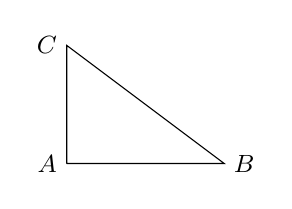
\begin{tikzpicture}[font=\small,x=5mm, y=5mm]

\draw (0,0)-- (4,0)--(0,3)--(0,0);

 \begin{scope}[left]
\node  at (0,3) {$C$};
\node  at (0,0) {$A$};
\end{scope}

\node[right]  at (4,0) {$B$};

\end{tikzpicture}% -----------------
